\section{The ladder and the quasi Riemann abscissa}\label{mi:sec:quasi}

The ladder $F_b$ of Section~\ref{mi:sec:ladder} is the opposite symmetrisation: $F_b=\cos(b\partial)\Xi$ while $g_b=\sec(b\partial)\Xi$, and in the Mellin variable $F_b(z)=\frac14\E[\Upsilon^s(\Upsilon^b+\Upsilon^{-b})]$ with $s=\frac12+iz$, the Rademacher Esscher weight in place of the logistic coin. On $\R$, $F_b(x)=\re\xi(\alpha+ix)$ with $\alpha=\frac12+b$. Theorem~\ref{mi:thm:ladder} is due to de Bruijn and Lagarias, who also showed that on $\RH$ all rungs $b>0$ are real rooted (Theorem~\ref{pol:thm:cosh}). We now locate the bottom rung $B_{\cosh}$. Let $\sigma_{\max}=\sup\{\re\rho\}$ over the nontrivial zeros of $\zeta$, and let $\gamma_k(b)$ be as in Theorem~\ref{mi:thm:ladder}.

\begin{proposition}\label{mi:prop:BTheta}
$B_{\cosh}\le\sigma_{\max}-\frac12$.
\end{proposition}

\begin{proof}
The zeros of $\Xi$ satisfy $|\im t|\le\Delta=\sigma_{\max}-\frac12$. De Bruijn's strip theorem with $\Delta$ in place of $\frac12$ in the proof of Theorem~\ref{mi:thm:ladder} shows that the zeros of $F_b$ satisfy $|\im z|\le(\max(\Delta^2-b^2,0))^{1/2}$, so $F_b$ is real rooted for $b\ge\Delta$ (Theorem~\ref{pol:thm:cosh}(ii)).
\end{proof}

Numerically, below height $100$ the number of real zeros of $\re\xi(\alpha+it)$ is $29=N(100)$ for every $\alpha\in\{0.5,0.55,0.6,0.7,0.8,1,1.25,1.5\}$ tested, and the first twelve Thorin atoms $\gamma_k(b)$, which move continuously where the zeros are simple, decrease strictly in $b$ on the grid $\alpha=0.50,0.51,\dots,1.00$ (Figure~\ref{mi:fig:path}); the smallest gap $\gamma_{k+1}-\gamma_k$ is $1.77$.

\begin{figure}[ht]
\centering
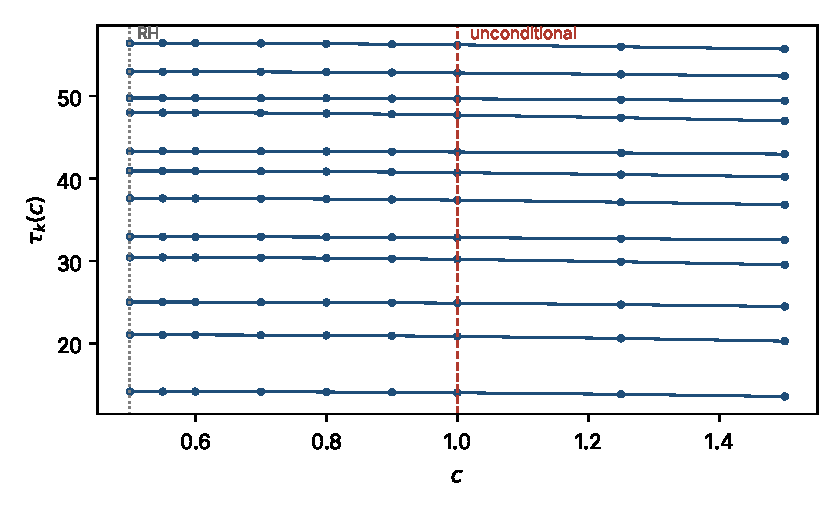
\includegraphics[width=\textwidth]{fig/mi_thorin_path.pdf}
\caption{The Thorin path: the first twelve atoms $\gamma_k(b)$ against $\alpha=\frac12+b$ at the stored values $\alpha=1,0.9,0.8,0.7,0.6,0.55,0.5$, from the unconditional rung $\alpha=1$ to the critical line.}
\label{mi:fig:path}
\end{figure}

Conversely, at height $x$ and $z=x+iy$ with $y>0$, Stirling and the functional equation give
\[
\frac{|\Xi(z+ib)|}{|\Xi(z-ib)|}\approx\Big(\frac x{2\pi}\Big)^{y}\frac{|\zeta(\alpha+y+ix)|}{|\zeta(\alpha-y+ix)|},
\]
so the two terms of $F_b$ can cancel off the axis only near zeros of $\zeta$ with $\beta\approx\alpha+y$, and, heuristically, Rouch\'e near a simple zero with $\beta>\alpha$ produces a zero of $F_b$ near $\gamma+i(\beta-\alpha)$. The cosh shift moves the effective abscissa by the fixed amount $b$; the heat flow, in the Rodgers Tao approximation, moves it by $\lambda\log(x/2\pi)$, which clears every zero at large height and is why Ki, Kim and Lee \cite{KKL09} have only finitely many nonreal zeros for every $\lambda>0$ and the Polymath bound \cite{Polymath} is reachable.

\begin{conjecture}\label{mi:conj:quasi}
Let $\sigma_{\max}^\infty=\limsup_{\gamma\to\infty}\beta$. Then $\sigma_{\max}^\infty-\frac12\le B_{\cosh}\le\sigma_{\max}-\frac12$. The upper bound is Proposition~\ref{mi:prop:BTheta}; the lower bound is conjectured. Under the conjecture, lowering the unconditional bound $B_{\cosh}\le\frac12$ is equivalent to a quasi Riemann hypothesis whenever $\sigma_{\max}$ is approached at large height.
\end{conjecture}

The mechanism can be tested on a function with genuine off line zeros. Let $\chi$ be the character modulo $5$ with $\chi(2)=i$ and $\kappa=(\sqrt{10-2\sqrt5}-2)/(\sqrt5-1)=0.2840790438$. The Davenport Heilbronn function \cite{DH36} is $f(s)=\frac{1-i\kappa}2L(s,\chi)+\frac{1+i\kappa}2L(s,\bar\chi)$, completed as $\Lambda(s)=(5/\pi)^{s/2}\Gamma(\frac{s+1}2)f(s)$; it satisfies $\Lambda(s)=\Lambda(1-s)$ (to $2.4\times10^{-29}$ at $30$ digits) and is real on the critical line, and its first zero off the line is $0.80851718246+85.69934848538i$. The ladder built from $\Lambda$ has a nonreal pair above this zero for $\alpha$ up to about $0.798$, slightly below $\beta$. The imaginary part of the pair is $0.2893$, $0.2244$, $0.1019$, $0.0685$, $0.0425$ at $\alpha=0.6$, $0.7$, $0.78$, $0.79$, $0.795$, and its square falls almost linearly near the collision (the slopes of the square are $-0.33$, $-0.50$, $-0.57$, $-0.57$ between consecutive values). The pair collides on the axis at $\alpha\approx0.798$ (the double root is at $\alpha=0.798095$, $x=85.6255$), and is real for $\alpha\ge0.80$, with the total count of zeros in the box $[83,88.5]\times[-0.9,0.9]$ conserved at $4$. The small early collision is a finite height effect, since $(x/2\pi)^y$ is only $13.6^y$ at height $85$; it is the reason for $\sigma_{\max}^\infty$ rather than $\sigma_{\max}$ in the lower bound.

\subsection{An exact paired form}\label{mi:sec:paired}

The ladder uses only the real part of $\xi$ on the vertical line. Pairing it with the imaginary part gives an exact statement. For $\alpha>\frac12$ put $E_\alpha(z)=\xi(\alpha-iz)$, $A_\alpha=\frac12(E_\alpha+E_\alpha^\#)$ and $B_\alpha=\frac i2(E_\alpha-E_\alpha^\#)$, with $E^\#(z)=\overline{E(\bar z)}$, so that $A_\alpha(t)=\re\xi(\alpha+it)=F_{\alpha-1/2}(t)$ and $B_\alpha(t)=\im\xi(\alpha+it)$ for real $t$, and $E_\alpha=A_\alpha-iB_\alpha$. Here $A_\alpha$ is the even part of Section~\ref{pol:sec:cosh} evaluated at $iz$.

\begin{theorem}\label{mi:thm:paired}
For $\alpha>\frac12$ the following are equivalent: (i) $\zeta(s)\ne0$ for $\re s\ge\alpha$; (ii) $E_\alpha$ is Hermite Biehler, that is $|E_\alpha(z)|>|E_\alpha^\#(z)|$ for $\im z>0$; (iii) $\re\xi(\alpha+it)$ and $\im\xi(\alpha+it)$, as entire functions of $t$, have only real simple zeros, and these strictly interlace. Hence the paired bottom rung, the infimum of the $\alpha-\frac12$ for which these hold, is exactly $\sigma_{\max}-\frac12$, and $\RH$ holds if and only if (iii) holds for every $\alpha>\frac12$.
\end{theorem}

\begin{proof}
(i)$\Rightarrow$(ii): for $z=x+iy$ with $y>0$ we have $E_\alpha(z)=\xi(\alpha+y-ix)$ and $E_\alpha^\#(z)=\xi(\alpha-y+ix)$. Let $\rho=\beta+i\gamma$ run over the zeros of $\xi$, a set symmetric under $\rho\mapsto\bar\rho$. By the Hadamard product, pairing $\rho$ with $\bar\rho$,
\[
\frac{|E_\alpha(z)|^2}{|E_\alpha^\#(z)|^2}=\prod_\rho\frac{(\alpha+y-\beta)^2+(x-\gamma)^2}{(\alpha-y-\beta)^2+(x-\gamma)^2}=\prod_\rho\Big(1+\frac{4y(\alpha-\beta)}{|\alpha-y+ix-\rho|^2}\Big),
\]
and every factor exceeds $1$ when $\beta<\alpha$. The product converges absolutely because $\sum\gamma^{-2}<\infty$, and $E_\alpha$ has no real zeros since no $\beta$ equals $\alpha$. Hence $|E_\alpha|>|E_\alpha^\#|$ on the upper half plane. (ii)$\Rightarrow$(iii) is the Hermite Biehler theorem in de Branges's form: if $E=A-iB$ is Hermite Biehler, then $A$ and $B$ are real entire with only real simple zeros that strictly interlace. (iii)$\Rightarrow$(i): $A_\alpha$ and $B_\alpha$ are real entire of order one with only real zeros, hence of genus at most one; $A_\alpha$ is even and $B_\alpha$ is odd, so their Hadamard products carry no factor $e^{az}$: $A_\alpha(z)=\xi(\alpha)\prod_k(1-z^2/a_k^2)$ and $B_\alpha(z)=\xi'(\alpha)z\prod_k(1-z^2/b_k^2)$ (without the parity the step fails, since interlacing alone allows an extra factor $e^{az}$). For strictly interlacing zeros the quotient of these products is, up to sign, a Pick function by Chebotarev's theorem \cite{Chebotarev28}. Since $B_\alpha/A_\alpha\sim(\xi'(\alpha)/\xi(\alpha))z$ at $0$, with $\xi(\alpha)>0$ and $\xi'(\alpha)>0$ ($\xi'(\alpha)>0$ holds unconditionally for $\alpha>\frac12$, because $\xi'/\xi(\alpha)=\sum_\rho(\alpha-\rho)^{-1}$ is real and each pair $\rho$, $1-\rho$ contributes $\re\big[(\alpha-\rho)^{-1}+(\alpha-1+\rho)^{-1}\big]=(2\alpha-1)(xy+\gamma^2)/((x^2+\gamma^2)(y^2+\gamma^2))>0$, with $x=\alpha-\beta$, $y=\alpha-1+\beta$ and $xy>-\frac14>-\gamma^2$), the sign is $+$: $B_\alpha/A_\alpha$ is a Pick function and $\im(B_\alpha/A_\alpha)>0$ on the upper half plane. The identity $|E_\alpha^\#|^2-|E_\alpha|^2=-4|A_\alpha|^2\im(B_\alpha/A_\alpha)$ then gives $|E_\alpha|>|E_\alpha^\#|\ge0$ on the upper half plane, and $E_\alpha\ne0$ on $\R$ because the zeros of $A_\alpha$ and $B_\alpha$ are disjoint. So $E_\alpha(z)=\xi(\alpha-iz)$ has no zeros in the closed upper half plane; since $E_\alpha(z)=0$ at $z=-\gamma+i(\beta-\alpha)$, this says $\beta<\alpha$ for every zero. (The other sign is excluded by Hardy: $E_\alpha^\#(z)=\xi(\alpha+iz)$ vanishes at $\gamma+i(\alpha-\frac12)$ for every zero on the line, so it is not Hermite Biehler.) The last two statements follow.
\end{proof}

In the language of de Branges spaces this is a statement about the function $E_\alpha$; its Thorin form is the following. Since $A_\alpha$ is even with $A_\alpha(0)=\xi(\alpha)>0$ and $B_\alpha$ is odd with $B_\alpha'(0)=\xi'(\alpha)>0$,
\[
\frac{2\xi(\alpha)}{\xi(\alpha+\sqrt s)+\xi(\alpha-\sqrt s)}\quad\text{and}\quad\frac{2\sqrt s\,\xi'(\alpha)}{\xi(\alpha+\sqrt s)-\xi(\alpha-\sqrt s)}
\]
(these are $\xi(\alpha)/A_\alpha(i\sqrt s)$ and $B_\alpha'(0)/(B_\alpha(z)/z)$ at $z=i\sqrt s$) are Laplace transforms of generalised gamma convolutions with strictly interlacing Thorin atoms exactly when $\zeta$ has no zeros with $\re s\ge\alpha$. Call two such generalised gamma convolutions, whose Thorin atoms $a_k^2$ and $b_k^2$ strictly interlace, a Thorin pair: the even and odd parts of $\xi$ about $\alpha$ form a Thorin pair precisely to the right of every zero. For $\zeta$ the interlacing holds on $[0,100]$ at $\alpha=0.55$, $0.6$, $0.7$, $1$ (and $0.8$, $1.25$, $1.5$), with $29$ positive zeros of each function and smallest distance between a zero of $A_\alpha$ and one of $B_\alpha$ equal to $0.50$, $0.51$, $0.54$, $0.69$ for $\alpha=0.55$, $0.6$, $0.7$, $1$. For Davenport Heilbronn the criterion is sharp where the ladder alone is not: at $\alpha=0.800$ and $0.805$ the real part already has only real zeros on $(83,88.5)$, yet the zeros of the real (A) and imaginary (B) parts come in the order ABAABBAB, while at $\alpha=0.82$ and $0.85$ the order is ABABABAB.
% UNCHECKED: Lagarias, de Branges spaces: the paper in which the Hermite Biehler form for xi is implicit (the source gives no reference; Lagarias05 is not it)

\subsection{Density one by phase counting}\label{mi:sec:density}

Let $\theta_\alpha(t)=\arg\xi(\alpha+it)$; for $\alpha>\sigma_{\max}$ this is $\pi$ times the clock $U_\alpha$ of Proposition~\ref{pol:prop:round}. Since $\re(\xi'/\xi)(s)=\sum_\rho\re(s-\rho)^{-1}$ (Hadamard's product; the same identity is used in the proof of Proposition~\ref{pol:prop:round}),
\[
\theta_\alpha'(t)=\sum_\rho\frac{\alpha-\beta}{(\alpha-\beta)^2+(t-\gamma)^2},
\]
a sum of Cauchy bumps of mass $+\pi$ for $\beta<\alpha$ and $-\pi$ for $\beta>\alpha$. Write $N^\pm(T)$ for the number of zeros with $|\gamma|\le T$ (so $N^\pm=2N$ with the usual $N$ counting $0<\gamma\le T$) and $N^\pm_{>\alpha}(T)$ for those with $\beta>\alpha$.

\begin{theorem}\label{mi:thm:density}
Let $\alpha>\frac12$ with $\beta\ne\alpha$ for every zero. Then $\theta_\alpha(T)-\theta_\alpha(-T)=\pi(N^\pm(T)-2N^\pm_{>\alpha}(T))+O(\log T)$. Hence $\re\xi(\alpha+it)$ and $\im\xi(\alpha+it)$ each have at least $N^\pm(T)-2N^\pm_{>\alpha}(T)-O(\log T)$ real zeros in $[-T,T]$. If moreover $F_b$, $b=\alpha-\frac12$, satisfies the Riemann von Mangoldt formula with error $O(\log T)$, its nonreal zeros with $|\re z|\le T$ number at most $2N^\pm_{>\alpha}(T)+O(\log T)$.
\end{theorem}

\begin{proof}
Integrating $\theta_\alpha'$ over $[-T,T]$, a zero $\rho$ with $|\gamma|\le T$ contributes $\operatorname{sgn}(\alpha-\beta)\,(\arctan\frac{T-\gamma}{|\alpha-\beta|}+\arctan\frac{T+\gamma}{|\alpha-\beta|})$, which is $\pm\pi$ up to a remainder of size $|\alpha-\beta|/(T-|\gamma|)$, and a zero with $|\gamma|>T$ contributes a remainder of size $|\alpha-\beta|/(|\gamma|-T)$, of the opposite sign. Zeros within distance $1$ of $\pm T$ number $O(\log T)$ and contribute $O(\log T)$ in all. The remaining remainders sum to $O(\log^2T)$ if estimated separately; pair $\rho$ with $1-\rho$, which has the same ordinate and combined weight $(\alpha-\beta)+(\alpha-1+\beta)=2\alpha-1$, independent of $\beta$. Up to $O(\log T)$ the remainders are then $(2\alpha-1)\sum_\gamma\operatorname{sgn}(|\gamma|-T)\big(\frac1{||\gamma|-T|}-\frac1{|\gamma|+T}\big)$, and partial summation with $N^\pm(t)=\frac t\pi\log\frac t{2\pi e}+O(\log t)$ shows that the contributions from below and from above $T$ cancel to $O(\log T)$. This proves the first formula. A continuous phase $\theta_\alpha$ with total change $\Delta$ crosses the lattice $\pi\mathbb Z$ (zeros of $\im\xi(\alpha+it)$) and the lattice $\pi\mathbb Z+\frac\pi2$ (zeros of $\re\xi(\alpha+it)$) at least $|\Delta|/\pi-1$ times each, with $\Delta=\theta_\alpha(T)-\theta_\alpha(-T)$. Under the Riemann von Mangoldt formula $F_b$ has $N^\pm(T)+O(\log T)$ zeros with $|\re z|\le T$, of which at least $N^\pm(T)-2N^\pm_{>\alpha}(T)-O(\log T)$ are real.
\end{proof}

With Ingham's estimate \cite{Ingham40}, $N^\pm_{>\alpha}(T)=O(T^{3(1-\alpha)/(2-\alpha)}\log^5T)=o(T)$ for every $\alpha=\frac12+b>\frac12$, since $3(1-\alpha)/(2-\alpha)<1$. So, unconditionally, $\re\xi(\alpha+it)$ has at least $N^\pm(T)-o(T)$ real zeros in $[-T,T]$, against $N^\pm(T)\sim\frac T\pi\log\frac T{2\pi}$ (this is the lower bound of the theorem). If the rung $F_b$ satisfies the Riemann von Mangoldt formula with error $O(\log T)$, which is open (Problem~\ref{mi:prob:rvm}), almost all zeros of $\frac12(\xi(s+b)+\xi(s-b))$ lie on the critical line, and as a count the number of conjugate pairs of nonreal zeros up to height $T$ is at most $N^\pm_{>\alpha}(T)+O(\log T)$. For the Davenport Heilbronn function, whose zeros off the line below height $200$ have $\beta=0.8085$, $0.6508$, $0.5744$, $0.7243$ (computed in $0.52\le\re s\le1.5$, $0.1\le\im s\le200$, at heights $85.70$, $114.16$, $166.48$, $176.70$), the real part of $\Lambda(\alpha+it)$ has $130$, $130$, $126$, $124$ real zeros on $(0.5,200)$ at $\alpha=0.95$, $0.85$, $0.7$, $0.6$, where $0$, $0$, $2$, $3$ of those zeros lie to the right of $\alpha$: the deficits $4$ and $6$ are two real zeros per zero to the right, as the count predicts. A direct count of the nonreal zeros of $F_b$ was not run, so that the statement that each such zero costs one conjugate pair is established at the level of these counts only. For $\zeta$ itself, the error $\theta_\alpha(T)-\theta_\alpha(-T)-\pi N^\pm(T)$ at $T=20,40,60,80,100$ stays below $1.6$ for $\alpha=0.6$, $0.75$, $1$ (computed).

\subsection{Universal factors as vertical averages}\label{mi:sec:vertical}

Every universal factor acts as a vertical average, $\int_\R\Phi(u)\E\cosh(uX)e^{izu}\,du=\E\,\Xi(z+iX)$: the ladder is $X=\pm b$ and the de Bruijn Newman flow is $X=\sqrt{2\lambda}\,\mathcal N$ with $\mathcal N$ standard normal. Since $|\Xi(x+iu)|$ grows like $(x/2\pi)^{|u|/2}$, the average is dominated near the Esscher tilt location
\[
u^*(L)=\arg\max_u\big[\tfrac L2u+\log p_X(u)\big],\qquad L=\log\frac x{2\pi},
\]
which is $\lambda L$ for the Gaussian, Rodgers and Tao's effective abscissa, and $\operatorname{ess\,sup}X$ for bounded $X$. Below the asymptotic regime $\lambda L^2\gg1$ both flows obey the local model of a pair at $\pm i\eta$, $\eta=\beta-\frac12$: on $z^2+\eta^2$, $\cos(b\partial)$ gives $z^2+\eta^2-b^2$ and $e^{-\lambda\partial^2}$ gives $z^2+\eta^2-2\lambda$, so the model predicts $b_c=\eta$ and $\lambda_c=\eta^2/2$. The heat flow of $\Lambda$ is the flow by $e^{\lambda u^2}$ of its kernel $\varphi(u)=2(5/\pi)^{-1/2}e^{3u/2}\sum_{n\ge1}n\,(a\chi(n)+\bar a\bar\chi(n))\exp(-\pi n^2e^{2u}/5)$, $a=\frac{1-i\kappa}2$, which is even and gives $\Lambda(\frac12+ix)$ by its Fourier transform. Table~\ref{mi:tab:thr} compares the model with three Davenport Heilbronn zeros.
% merge-E2.md: kernel of the heat flow of Lambda taken from checks-G4.md (a, the coefficient of L(s,chi), inferred from the definition of f)

\begin{table}[ht]
\centering
\footnotesize
\setlength{\tabcolsep}{3.5pt}
\begin{tabular}{lcccccc}
\toprule
zero & $\eta$ & $L$ & $b_c$ & $b_c/\eta$ & $\lambda_c$ & $\lambda_c/(\eta^2/2)$\\
\midrule
$0.8085+85.699i$ & 0.3085 & 2.613 & 0.2981 & 0.966 & 0.0441 & 0.927\\
$0.6508+114.163i$ & 0.1508 & 2.900 & 0.1504 & 0.997 & 0.0111 & 0.978\\
$0.7243+176.702i$ & 0.2243 & 3.337 & 0.2190 & 0.977 & 0.0237 & 0.941\\
\bottomrule
\end{tabular}
\caption{Critical ladder rung $b_c$ and heat time $\lambda_c$ at which the pair above each Davenport Heilbronn zero becomes real. In every case $\lambda_cL^2<1$ ($0.30$, $0.09$, $0.26$), so these heights are pre asymptotic for the heat flow.}
\label{mi:tab:thr}
\end{table}

For $\zeta$, where an off line zero would lie above $3\times10^{12}$ \cite{PT21} ($L\approx27$), the heat flow would absorb a zero at $\lambda\approx\eta/L$, far below the local value $\eta^2/2$ once $\eta>2/L$ (with $L=26.89$, $2/L=0.074$), while the ladder needs $b\approx\eta$. In this local model the cosh ladder, unlike the de Bruijn Newman constant, admits no Polymath style improvement short of a quasi Riemann hypothesis.

\section{Open problems}\label{mi:sec:open}

The computations of this chapter leave the following questions, from the friable approximants of Section~\ref{mi:sec:miyatake} to the ladder of Section~\ref{mi:sec:quasi}. The scripts that produce the numbers of the chapter are listed in \texttt{code/README.md} of the repository of the book.

\begin{problem}
Decide whether the heuristic of Remark~\ref{mi:prop:zerocount} holds with a bounded error.
\end{problem}

\begin{problem}\label{mi:prob:nuP}
Assuming $\RH$ for $\Xi$, decide whether $\nu_P\ge0$ on all of $(0,\infty)$ for every $P$. The angle $y_0/x_0\sim(\pi/2)/\log x_0$ of the departed chain tends to zero, which suggests yes; the computed range is $[0.02,3]$.
\end{problem}

\begin{problem}
Prove Conjecture~\ref{mi:conj:survey}, or at least $|R_P-N(\tau_P^*)|=O(\log q)$ under $\RH$ and a lower bound for the peaks of Hardy's function $Z$ on negative humps.
\end{problem}

\begin{problem}
Find a computable Thorin criterion that detects the departed zeros, for instance the failure of positivity of Hankel or moment matrices built from $\nu_P$ beyond a certain order, and use the friable approximants to calibrate it.
\end{problem}

\begin{problem}
Prove that all zeros of $g^{(2)}$ lie in $|\im w|<2$, and deduce from de Bruijn's theorem that every zero of Miyatake's $\xi^{(2)}$ is real.
\end{problem}

\begin{problem}
Prove that no factorisation $\Phi=U\chi$ with $U=\E\cosh(tX)$ a nontrivial universal factor has $\hat\chi$ in the Laguerre P\'olya class, which would extend the theorem of Rodgers and Tao from Gaussian factors to Cardon's factors.
\end{problem}

\begin{problem}\label{mi:prob:quasi}
Make the local mechanism of Section~\ref{mi:sec:quasi} rigorous at all large heights, proving $B_{\cosh}\ge\sigma_{\max}^\infty-\frac12$ in Conjecture~\ref{mi:conj:quasi}; Theorem~\ref{mi:thm:paired} already settles the paired version.
\end{problem}

\begin{problem}\label{mi:prob:rvm}
Prove the Riemann von Mangoldt formula for the rungs $F_b$ with error $O(\log T)$, which makes the density one statement after Theorem~\ref{mi:thm:density} unconditional.
\end{problem}

\begin{problem}
Prove a Ki, Kim and Lee theorem for the vertical average $\E\,\Xi(z+iX)$ whenever $X$ is unbounded, and show that for bounded $X$ the nonreal zeros at large height sit above zeros of $\zeta$ with $\beta>\frac12+\operatorname{ess\,sup}X$.
\end{problem}

\begin{problem}\label{mi:prob:escape}
Make the escape law \eqref{mi:eq:escape} rigorous for $b>2$, $C_b\ne0$.
\end{problem}

\begin{problem}\label{mi:prob:b0}
Certify, by interval arithmetic, that $C_b$ has exactly one zero $b_0$ on $(2,\infty)$: an interval Newton enclosure of $b_0=2.4588641657$, the sign of $\Phi(i\pi/(2b))$ on $(2,20]$ by subdivision with a rigorous tail for the series over $n$, Theorem~\ref{mi:thm:cusp} with an explicit error near $b=2$, and a proof that $\Phi(iy)>0$ for $0<y\le\pi/40$ to cover $b>20$.
\end{problem}

\paragraph{Notes.} The identity \eqref{mi:eq:miyid} and the function $\xi^{(P)}$ with its Theorem I are Miyatake's \cite{Miyatake51b}, and the symmetrised kernel with a secant pole term is that of his paper A \cite{Miyatake51a}; Hejhal \cite{Hejhal90} treats truncated symmetrised kernels. The ladder is that of de Bruijn and Lagarias, the shift identity and the Brownian and Mellin readings of Section~\ref{mi:sec:prob} use the Biane Pitman Yor identity \cite{BPY01} and the P\'olya Gamma mixture of Polson, Scott and Windle \cite{PSW13}, the paired form uses Chebotarev's theorem \cite{Chebotarev28}, and the counting in Section~\ref{mi:sec:density} uses Ingham's density estimate \cite{Ingham40}. The statements about Miyatake's two papers rest on their description by the authors of the chapter and have not been checked against the papers.
